%% LyX 1.3 created this file.  For more info, see http://www.lyx.org/.
%% Do not edit unless you really know what you are doing.
\documentclass[11pt,english,english]{article}
\usepackage[T1]{fontenc}
\usepackage[latin1]{inputenc}
\usepackage{graphicx}

\makeatletter

%%%%%%%%%%%%%%%%%%%%%%%%%%%%%% LyX specific LaTeX commands.
\newcommand{\noun}[1]{\textsc{#1}}
%% Bold symbol macro for standard LaTeX users
\providecommand{\boldsymbol}[1]{\mbox{\boldmath $#1$}}


%%%%%%%%%%%%%%%%%%%%%%%%%%%%%% User specified LaTeX commands.
\usepackage[T1]{fontenc}
\usepackage[latin1]{inputenc}
\usepackage{geometry}
\geometry{verbose,a4paper,lmargin=2.5cm,rmargin=2cm}
\usepackage{babel}
\usepackage{graphics}
\usepackage{setspace}
\onehalfspacing

\makeatletter

\textwidth 16.2cm
\textheight 24.0cm
\oddsidemargin 0.5cm
\evensidemargin 0.5cm
\topmargin  0.5cm
\headheight 0cm
\makeatother

\usepackage{babel}
\makeatother
\begin{document}

\title{Molecular mechanics module}


\author{Aleksey M. Shor, \\
 Institute of Chemistry and Chemical Technology, \\
 Russian Academy of Sciences, Krasnoyarsk, Russian Federation}

\maketitle

\section{Introduction}

~~~~~Molecular mechanics module is a computer program to apply
molecular mechanics methods to geometry optimization of different
periodic and non-periodic systems and perform hybrid quantum mechanical-molecular
mechanical (QM/MM) calculations. It has been implemented as a part
of quantum mechanical package \noun{ParaGauss} that handles a molecular
mechanics run. Molecular mechanics module uses all data types and
interface procedures derived into \noun{ParaGauss} but has strong
independent structure and source code.


\section{Program abilities}

\begin{enumerate}
\item Molecular mechanics module can treat systems having 2-dimensional
and 3-dimensional periodicity and systems without periodicity at all.
\item Energy, gradients and second derivatives in respect to atom coordinates
are calculated.
\item For periodic systems (2-D and 3-D) first and second energy derivatives
in respect to elements of strain tensor also can be obtained.
\item Geometry optimization is based on Newton-Raphson method using analytical
Hessian and BFGS updating scheme. Also for large systems there is
possibility to avoid calculating analytical second derivatives and
use diagonal matrix as initial Hessian
\item Optimization of cell parameters is possible for periodic systems during
optimization of atom coordinates.
\item There is an interface between quantum mechanical part of \noun{ParaGauss}
and Molecular mechanics module to perform QM/MM task (IMOMM). 
\end{enumerate}

\section{Force field}

The potential functions implemented in Molecular mechanics module
based on MM3 force field for saturated hydrocarbons\cite{mm3} (slightly
extended variant) and can be divided in two parts:

\begin{enumerate}
\item \emph{Bonded} \emph{(covalent interactions)}: stretching, bending,
torsion and cross terms (stretching-stretching, bending-bending, stretching-bending,
stretching-torsion). 
\item \emph{Non-bonded (van der Waals and electrostatic interactions)}:
Lennard-Jones, Buckingham, van der Waals tabulated, point charges,
dipole-dipole. 
\end{enumerate}

\subsection{Bonded interactions}


\subsubsection{Stretching potentials}

~~~~~Harmonic:\begin{equation}
E\left(r_{ij}\right)=\frac{k2_{ij}}{2}\left(r_{ij}-r_{ij}^{0}\right)^{2}\label{eq:1}\end{equation}


Quartic:\begin{eqnarray}
E\left(r_{ij}\right) & = & \frac{k2_{ij}}{2}\left(r_{ij}-r_{ij}^{0}\right)^{2}+\frac{k3_{ij}}{3}\left(r_{ij}-r_{ij}^{0}\right)^{3}\nonumber \\
 & + & \frac{k4_{ij}}{4}\left(r_{ij}-r_{ij}^{0}\right)^{4}\label{eq:2}\end{eqnarray}


Morse:\begin{equation}
E\left(r_{ij}\right)=D_{ij}\left\{ \left[1-\exp\left(-A_{ij}\left(r_{ij}-r_{ij}^{0}\right)\right)\right]^{2}-1\right\} \label{eq:3}\end{equation}
Here $r_{ij}$ is the distance between atoms $i$ and $j$ at Cartesian
coordinates $\overrightarrow{r_{i}}$ and $\overrightarrow{r_{j}}$. 

The gradients on each atom taking part in a stretching interaction
are calculated using general formulas:\begin{eqnarray}
\overrightarrow{G}^{xyz}\left(i\right) & = & \frac{\partial E\left(r_{ij}\right)}{\partial r_{ij}}\frac{\overrightarrow{r}_{ij}^{xyz}}{r_{ij}}\nonumber \\
\overrightarrow{G}^{xyz}\left(j\right) & = & -\frac{\partial E\left(r_{ij}\right)}{\partial r_{ij}}\frac{\overrightarrow{r}_{ij}^{xyz}}{r_{ij}}\label{eq:36}\end{eqnarray}



\subsubsection{Bending potentials}

~~~~~Harmonic:\begin{equation}
E\left(\theta_{ijk}\right)=\frac{k2_{ijk}}{2}\left(\theta_{ijk}-\theta_{ijk}^{0}\right)^{2}\label{eq:4}\end{equation}


Quartic:\begin{eqnarray}
E\left(\theta_{ijk}\right) & = & \frac{k2_{ijk}}{2}\left(\theta_{ijk}-\theta_{ijk}^{0}\right)^{2}+\frac{k3_{ijk}}{3}\left(\theta_{ijk}-\theta_{ijk}^{0}\right)^{4}\nonumber \\
 & + & \frac{k4_{ijk}}{4}\left(\theta_{ijk}-\theta_{ijk}^{0}\right)^{4}\label{eq:5}\end{eqnarray}


Six:\begin{eqnarray}
E\left(\theta_{ijk}\right) & = & \frac{k2_{ijk}}{2}\left(\theta_{ijk}-\theta_{ijk}^{0}\right)^{2}+\frac{k3_{ijk}}{3}\left(\theta_{ijk}-\theta_{ijk}^{0}\right)^{4}\label{eq:6}\\
 & + & \frac{k4_{ijk}}{4}\left(\theta_{ijk}-\theta_{ijk}^{0}\right)^{4}+\frac{k5_{ijk}}{5}\left(\theta_{ijk}-\theta_{ijk}^{0}\right)^{5}\nonumber \\
 & + & \frac{k6_{ijk}}{6}\left(\theta_{ijk}-\theta_{ijk}^{0}\right)^{6}\nonumber \\
\nonumber \end{eqnarray}


$\theta_{ijk}$ is the angle between the distance vectors $\overrightarrow{r_{ij}}$
and $\overrightarrow{r_{kj}}$:\begin{equation}
\theta_{ijk}=\arccos\left(\frac{\overrightarrow{r}_{ij}\cdot\overrightarrow{r}_{kj}}{r_{ij}r_{kj}}\right)\label{eq:37}\end{equation}
Gradients on atoms derived from the bending potential are:\begin{eqnarray}
\overrightarrow{G}^{xyz}\left(i\right) & = & \frac{\partial E\left(\theta_{ijk}\right)}{\partial\theta_{ijk}}\frac{\left[\cos\left(\theta_{ijk}\right)\frac{\overrightarrow{r}_{ij}^{xyz}}{r_{ij}}-\frac{\overrightarrow{r}_{kj}^{xyz}}{r_{kj}}\right]}{r_{ij}\sin\left(\theta_{ijk}\right)}\nonumber \\
\overrightarrow{G}^{xyz}\left(j\right) & = & \frac{\partial E\left(\theta_{ijk}\right)}{\partial\theta_{ijk}}\frac{\left\{ \left[r_{ij}-r_{kj}\cos\left(\theta_{ijk}\right)\right]\frac{\overrightarrow{r}_{ij}^{xyz}}{r_{ij}}+\left[r_{kj}-r_{ij}\cos\left(\theta_{ijk}\right)\right]\frac{\overrightarrow{r}_{kj}^{xyz}}{r_{kj}}\right\} }{r_{ij}r_{kj}\sin\left(\theta_{ijk}\right)}\label{eq:38}\\
\overrightarrow{G}^{xyz}\left(k\right) & = & \frac{\partial E\left(\theta_{ijk}\right)}{\partial\theta_{ijk}}\frac{\left[\cos\left(\theta_{ijk}\right)\frac{\overrightarrow{r}_{kj}^{xyz}}{r_{kj}}-\frac{\overrightarrow{r}_{ij}^{xyz}}{r_{ij}}\right]}{r_{kj}\sin\left(\theta_{ijk}\right)}\nonumber \end{eqnarray}



\subsubsection{Torsion potentials}

~~~~~Harmonic:\begin{equation}
E\left(\varphi_{ijkl}\right)=\frac{k2_{ijkl}}{2}\left(\varphi_{ijkl}-\varphi_{ijkl}^{0}\right)^{2}\label{eq:7}\end{equation}


Triple cosine:\begin{eqnarray}
E\left(\varphi_{ijkl}\right) & = & \frac{k1_{ijkl}}{2}\left[1+\cos\left(\varphi_{ijkl}\right)\right]\nonumber \\
 & + & \frac{k2_{ijkl}}{2}\left[1-\cos\left(2\varphi_{ijkl}\right)\right]\label{eq:8}\\
 & + & \frac{k3_{ijkl}}{2}\left[1+\cos\left(3\varphi_{ijkl}\right)\right]\nonumber \\
\nonumber \end{eqnarray}
 

$\varphi_{ijkl}$ is the dihedral angle between the planes defined
by $\left\{ \overrightarrow{r_{ij}},\overrightarrow{r_{kj}}\right\} $
and $\left\{ \overrightarrow{r_{jk}},\overrightarrow{r_{lk}}\right\} $.
Gradients on atoms $i$, $j$, $k$ and $l$ arising from the 4-body
torsion potential are too complicated to be presented in the current
document.


\subsubsection{Cross terms}

~~~~~Stretching-stretching:\begin{equation}
E\left(r_{ij},r_{kj}\right)=\frac{k_{ijk}}{2}\left(r_{ij}-r_{ij}^{0}\right)\left(r_{kj}-r_{kj}^{0}\right)\label{eq:9}\end{equation}


Bending-bending:\begin{equation}
E\left(\theta_{ijk},\theta_{ljm}\right)=\frac{k_{ikjlm}}{2}\left(\theta_{ijk}-\theta_{ijk}^{0}\right)\left(\theta_{ljm}-\theta_{ljm}^{0}\right)\label{eq:10}\end{equation}


Stretching-bending:\begin{eqnarray}
E\left(r_{ij},r_{kj},\theta_{ijk}\right) & = & k_{ijijk}\left(r_{ij}-r_{ij}^{0}\right)\left(\theta_{ijk}-\theta_{ijk}^{0}\right)\nonumber \\
 & + & k_{kjijk}\left(r_{kj}-r_{kj}^{0}\right)\left(\theta_{ijk}-\theta_{ijk}^{0}\right)\label{eq:11}\end{eqnarray}


Stretching-torsion:\begin{equation}
E\left(r_{jk},\varphi_{ijkl}\right)=\frac{k_{ijkl}}{2}\left(r_{jk}-r_{jk}^{0}\right)\left[1+\cos\left(3\varphi_{ijkl}\right)\right]\label{eq:12}\end{equation}
Gradients on atoms taking part in crossing potentials can be easy
given as a combination of derivatives of stretching, bending and torsion
potentials.


\subsection{Non bonding interactions}


\subsubsection{Van der Waals interactions}

~~~~~Buckingham:\begin{equation}
E\left(r_{ij}\right)=A_{ij}\exp\left(-\frac{r_{ij}}{\rho_{ij}}\right)-\frac{C_{ij}}{r_{ij}^{6}}\label{eq:13}\end{equation}


Lennard-Jones:\begin{equation}
E\left(r_{ij}\right)=\frac{A_{ij}}{r_{ij}^{12}}-\frac{C_{ij}}{r_{ij}^{6}}\label{eq:14}\end{equation}


Tabulated potential:\begin{equation}
E\left(r_{ij}\right)=A_{ij}g\left(r_{ij}\right)+C_{ij}h\left(r_{ij}\right)\label{eq:17}\end{equation}
 $g\left(r\right)$ and $h\left(r\right)$ in equation \ref{eq:17}
are user defined functions. Note that $g\left(r\right)$ has to describe
a repulsion interaction and $h\left(r\right)$ presents a dispersion
term and consequently should be $<0$. Functions $g\left(r\right)$
and $h\left(r\right)$ are interpolated using cubic spline method.
The cubic interpolation looks like\begin{eqnarray}
f\left(r\right) & = & f_{i}+\delta\left\{ f_{i+1}-f_{i}-\frac{\Delta^{2}}{6}\left[2f_{i}^{\prime\prime}+f_{i+1}^{\prime\prime}\right]\right\} \nonumber \\
 & + & \delta^{3}\frac{\Delta^{2}}{6}(f_{i+1}^{\prime\prime}-f_{i}^{\prime\prime})\label{eq:18}\end{eqnarray}
 and $\Delta=r_{i+1}-r_{i}$, $\delta=(r-r_{i})/\Delta$. Note that
the $r$-dependence is completely in $\delta$.

The gradients on atoms derived from one of these potentials are calculated
by the standard equations:\begin{eqnarray}
\overrightarrow{G}^{xyz}\left(i\right) & = & \frac{\partial E\left(r_{ij}\right)}{\partial r_{ij}}\frac{\overrightarrow{r}_{ij}^{xyz}}{r_{ij}}\nonumber \\
\overrightarrow{G}^{xyz}\left(j\right) & = & -\frac{\partial E\left(r_{ij}\right)}{\partial r_{ij}}\frac{\overrightarrow{r}_{ij}^{xyz}}{r_{ij}}\label{eq:39}\end{eqnarray}



\subsubsection{Electrostatic interactions}

~~~~~Point charge - point charge interaction:

a) non-periodic case (direct Coulomb sum)

\begin{equation}
E\left(r_{ij}\right)=\frac{1}{4\pi\varepsilon_{0}}\frac{q_{i}q_{j}}{\varepsilon_{p}r_{ij}}\label{eq:15}\end{equation}
The electrostatic gradients on atoms $i$ and $j$ derived from direct
Coulomb sum are\begin{eqnarray}
\overrightarrow{G}^{xyz}\left(i\right) & = & \frac{1}{4\pi\varepsilon_{0}}\frac{q_{i}q_{j}}{\varepsilon_{p}r_{ij}^{2}}\frac{\overrightarrow{r}_{ij}^{xyz}}{r_{ij}}\nonumber \\
\overrightarrow{G}^{xyz}\left(i\right) & = & -\frac{1}{4\pi\varepsilon_{0}}\frac{q_{i}q_{j}}{\varepsilon_{p}r_{ij}^{2}}\frac{\overrightarrow{r}_{ij}^{xyz}}{r_{ij}}\label{eq:40}\end{eqnarray}


b) 3-D periodic systems (classical Ewald method\cite{ewald3})\begin{eqnarray}
E & = & \frac{1}{4\pi\varepsilon_{0}}\sum_{\overrightarrow{n}}\sum_{i=1}^{N}\sum_{j=i+1}^{N}q_{i}q_{j}\frac{erfc\left(\alpha\left|\overrightarrow{r_{ij}}+\overrightarrow{n}\right|\right)}{\left|\overrightarrow{r_{ij}}+\overrightarrow{n}\right|}\nonumber \\
 & + & \frac{1}{\varepsilon_{0}V}\sum_{\overrightarrow{k}>0}\frac{\exp\left(-\frac{k^{2}}{4\alpha^{2}}\right)}{k^{2}}\left\{ \left|\sum_{i=1}^{N}q_{i}\cos\left(\overrightarrow{k}\cdot\overrightarrow{r_{i}}\right)\right|^{2}\right.\label{eq:19}\\
 & + & \left.\left|\sum_{i=1}^{N}q_{i}\sin\left(\overrightarrow{k}\cdot\overrightarrow{r_{i}}\right)\right|^{2}\right\} -\frac{1}{4\pi\varepsilon_{0}}\frac{\alpha}{\sqrt{\pi}}\sum_{i=1}^{N}q_{i}^{2}\nonumber \end{eqnarray}
The gradient on an atom $j$ is obtained by differentiation of equation
\ref{eq:19}:\begin{eqnarray}
\overrightarrow{G}^{xyz}\left(j\right) & = & -\frac{1}{4\pi\varepsilon_{0}}\sum_{\overrightarrow{n}}\sum_{i=1}^{N}q_{i}q_{j}\left\{ \frac{erfc\left(\alpha\left|\overrightarrow{r_{ij}}+\overrightarrow{n}\right|\right)}{\left|\overrightarrow{r_{ij}}+\overrightarrow{n}\right|^{2}}\right.\nonumber \\
 & + & \left.\frac{2\alpha\exp\left(-\alpha^{2}\left|\overrightarrow{r_{ij}}+\overrightarrow{n}\right|^{2}\right)}{\sqrt{\pi}\left|\overrightarrow{r_{ij}}+\overrightarrow{n}\right|}\right\} \frac{\left(\overrightarrow{r}_{ij}+\overrightarrow{n}\right)^{xyz}}{\left|\overrightarrow{r}_{ij}+\overrightarrow{n}\right|}\label{eq:41}\\
 & - & \frac{1}{\varepsilon_{0}V}\sum_{\overrightarrow{k}>0}\frac{\overrightarrow{k}^{xyz}\exp\left(-\frac{k^{2}}{4\alpha^{2}}\right)}{k^{2}}\left\{ \sin\left(\overrightarrow{k}\cdot\overrightarrow{r_{j}}\right)\right.\nonumber \\
 & \times & \left.\sum_{i=1}^{N}\cos\left(\overrightarrow{k}\cdot\overrightarrow{r_{i}}\right)-\cos\left(\overrightarrow{k}\cdot\overrightarrow{r_{j}}\right)\sum_{i=1}^{N}\sin\left(\overrightarrow{k}\cdot\overrightarrow{r_{i}}\right)\right\} \nonumber \end{eqnarray}


c) 2-D periodic systems (2-D variant of Ewald method\cite{parry,ewald2})\begin{eqnarray}
E & = & \frac{1}{4\pi\varepsilon_{0}}\sum_{\overrightarrow{m}}\sum_{i=1}^{N}\sum_{j=i+1}^{N}q_{i}q_{j}\frac{erfc\left(\alpha\left|\overrightarrow{r_{ij}}+\overrightarrow{m}\right|\right)}{\left|\overrightarrow{r_{ij}}+\overrightarrow{m}\right|}\nonumber \\
 & + & \frac{1}{4\pi\varepsilon_{0}}\sum_{i=1}^{N}\sum_{j=i+1}^{N}\sum_{\overrightarrow{h}>0}\frac{\pi\cos\left(\overrightarrow{h}\cdot\overrightarrow{r_{ij}}\right)}{hA}\nonumber \\
 & \times & \left\{ \exp\left(hz_{ij}\right)erfc\left(\alpha z_{ij}+\frac{h}{2\alpha}\right)+\exp\left(-hz_{ij}\right)\right.\label{eq:20}\\
 & \times & \left.erfc\left(-\alpha z_{ij}+\frac{h}{2\alpha}\right)\right\} -\frac{1}{4\pi\varepsilon_{0}}\sum_{i=1}^{N}\sum_{j=i+1}^{N}q_{i}q_{j}\frac{2\pi}{A}\nonumber \\
 & \times & \left\{ z_{ij}erf\left(\alpha z_{ij}\right)+\frac{1}{\alpha\sqrt{\pi}}\exp\left[-\left(\alpha z_{ij}\right)^{2}\right]\right\} \nonumber \\
 & - & \frac{1}{4\pi\varepsilon_{0}}\frac{\alpha}{\sqrt{\pi}}\sum_{i=1}^{N}q_{i}^{2}\nonumber \end{eqnarray}
For 2-D Ewald method it is reasonable to present the contribution
to the gradient on an atom $j$ only reciprocal-space part, because
real space contribution to the gradient looks absolutely the same
excluding the summation over a slab:\begin{eqnarray}
\overrightarrow{G}_{recip}^{xy}\left(j\right) & = & -\frac{1}{4\pi\varepsilon_{0}}\sum_{i=1}^{N}\sum_{h>0}\frac{\overrightarrow{h}^{xy}\pi\sin\left(\overrightarrow{h}\cdot\overrightarrow{r_{ij}}\right)}{hA}\nonumber \\
 & \times & \left\{ \exp\left(hz_{ij}\right)erfc\left(\alpha z_{ij}+\frac{h}{2\alpha}\right)+\exp\left(-hz_{ij}\right)\right.\nonumber \\
 & \times & \left.erfc\left(-\alpha z_{ij}+\frac{h}{2\alpha}\right)\right\} \nonumber \\
\overrightarrow{G}_{recip}^{z}\left(j\right) & = & \frac{1}{4\pi\varepsilon_{0}}\sum_{i=1}^{N}\sum_{h>0}\frac{\pi\cos\left(\overrightarrow{h}\cdot\overrightarrow{r_{ij}}\right)}{hA}\label{eq:42}\\
 & \times & \left\{ h\exp\left(hz_{ij}\right)erfc\left(\alpha z_{ij}+\frac{h}{2\alpha}\right)-\frac{2\alpha}{\sqrt{\pi}}\exp\left(hz_{ij}\right)\right.\nonumber \\
 & \times & \exp\left(-\left[\alpha z_{ij}+\frac{h}{2\alpha}\right]^{2}\right)-h\exp\left(-hz_{ij}\right)erfc\left(-\alpha z_{ij}+\frac{h}{2\alpha}\right)\nonumber \\
 & + & \left.\frac{2\alpha}{\sqrt{\pi}}\exp\left(-hz_{ij}\right)\exp\left(-\left[-\alpha z_{ij}+\frac{h}{2\alpha}\right]^{2}\right)\right\} \nonumber \\
 & - & \frac{1}{4\pi\varepsilon_{0}}\sum_{i=1}^{N}q_{i}q_{j}\frac{2\pi}{A}\left\{ erf\left(\alpha z_{ij}\right)+z_{ij}\frac{4\alpha}{\sqrt{\pi}}\exp\left(-\alpha^{2}z_{ij}^{2}\right)\right\} \nonumber \end{eqnarray}


In equations \ref{eq:19} and \ref{eq:20} $\overrightarrow{n}$ and
$\overrightarrow{m}$ are lattice vectors in a real-space for 3-D
and 2-D systems, respectively, and $\overrightarrow{k}$ and $\overrightarrow{h}$
are lattice vectors in a reciprocal-space, respectively. $n$, $m$,
$k$ and $h$ are their corresponding moduli. $N$ is the total number
of charged atoms. $V$ and $A$ are the volume and the area of 3-D
and 2-D unit cell, respectively. $\alpha$ is the parameters that
controls the contribution and the convergence of sums in a real- and
reciprocal-spaces. Ewald sum generally scales as $N^{2}$\cite{parry},
but for 3-D variant $N^{3/2}$ scaling can be achieved by choosing
optimal value of $\alpha$\cite{fincham,jackson}. Selection of this
value is based on the criterion of minimizing the total number of
terms to be calculated in real- and reciprocal-space, weighted by
relative computational time for the operations involved, $w$\cite{jackson}:\begin{equation}
\alpha^{2}=\left(\frac{Nw\pi^{3}}{V^{2}}\right)^{\frac{1}{6}}\label{eq:31}\end{equation}
For 2-D Ewald method $\alpha=1.2/\sqrt{A}$ is reasonable choice\cite{ewald2}.

Dipole - dipole interaction\cite{mm2} (figure \ref{cap:2}):\begin{equation}
E\left(R_{ij}\right)=f_{d}\frac{d_{i}d_{j}}{\varepsilon_{d}R_{ij}^{3}}\left[\cos\left(\chi_{ij}\right)-3\cos\left(\alpha_{ij}\right)\cos\left(\beta_{ij}\right)\right]\label{eq:16}\end{equation}


%
\begin{figure}
\begin{center}\includegraphics[%
  width=4cm,
  height=4cm]{dip_dip.eps}\end{center}


\caption{\label{cap:2}Definition of dipole-dipole interaction}
\end{figure}



\section{Definition of N-body lists}

~~~~~To save computational time during optimization process the
calculations of each contribution to the total energy, gradients and
Hessian of system are based on \texttt{\textbf{N-body lists}}. 


\subsection{Bonded interactions}

~~~~~For bonded (covalent) interactions \texttt{\textbf{N-body
lists}} are constructed only once in the beginning of a computational
task. There are two different possibilities to define bonded \texttt{\textbf{N-body
lists}}. The first method is automatic. It is based on predefined
or user specified covalent atom radii to calculate connectivity of
atoms and used potential functions. In the current version of Molecular
mechanics module only lists of 2- and 3-body bonded interactions can
be constructed by means the automatic procedure. 

The second way is more general and is used in the most part of molecular
mechanics and molecular dynamics packages\cite{amber,charmm,dl_poly,ego,gromacs}.
An user has to define \texttt{\textbf{N-body lists}} by hand for each
type of bonded interactions. Of course, this job is not simple and
even for relatively small systems demands great attentiveness from
anyone. Opposite some other molecular simulation packages the definition
of \texttt{\textbf{N-body lists}} in Molecular mechanics module is
separated from the definition of potential functions. The advantages
of this approach are that (1) an input file is now much more flexible,
because once specified potential functions can be very easy applied
for another similar molecular systems as include file and (2) constructing
\texttt{\textbf{N-body lists}} are simpler, because there is no necessity
to determine a correspondence between each set of interacting atoms
and acting potential. \texttt{\textbf{N-body lists}} has to be inputted
for all specified different types of covalent interactions (stretching,
bending, torsion, stretching-bending and etc.). \texttt{\textbf{}}

\texttt{\textbf{N-body lists}} are potential lists. It means they
are constructed for each specified bonded potential not atoms.


\subsection{Non-bonded interactions}

~~~~~Non bonded pair interactions consist of van der Waals and
Coulomb potentials. Unlike potentials modeling covalent interactions
between nearest atoms they are not local. Coulomb forces generally
act between all atoms consisting a system under study that is due
to their slow convergence. Van der Waals interactions are more local
than electrostatic one and it is a common rule to calculate short-range
non bonded energy and forces acting on a each atom as a result of
interaction with all other atoms located inside a sphere with the
cutoff radius $R_{cut}$. Numbers of these atoms are formed \texttt{\textbf{pair
lists}} for each atom taking part in van der Waals interactions.

The most part of force fields derived to model covalent molecular
systems exclude as rule any non-bonded interaction between atoms taking
part in bonded 2-, 3- and (sometimes) 4-body interactions\cite{mm3}.
In modeling a polarization of solids by shell-model non-bonded interactions
between core and shell of the same atom also has to be excluded. Atoms
that have to be excluded from non-bonded interactions are formed so-called
\texttt{\textbf{excluded list}}. Like bonded \texttt{\textbf{N-body
lists excluded list}} is constructed only once in the beginning of
a molecular mechanics task for each an atom of simulated system and
never recalculated because that is due to its covalent nature.

A content of non-bonded \texttt{\textbf{pair lists}} usually is not
constant value and depends on atomic positions during optimization
process. To avoid problems of unreasonable energy jumping between
different geometry configurations non-bonded \texttt{\textbf{pair
lists}} has to be recalculated during a structural optimization. In
current version of Molecular mechanics module non-bonded \texttt{\textbf{pair
lists}} are recalculated before each optimization geometry step. This
periodicity is the most suitable for systems consisting of some thousand
atoms. 

As it was mentioned above an electrostatic energy and forces have
very slow convergence in space. To calculate Coulomb interaction of
isolated molecular systems no any geometry limitations (cut-off radius
$R_{cut}$) are used. This rule in Molecular mechanics module is applied
to treat molecular system described by usual point charges and also
bond dipoles though it is well known that a dipole-dipole interaction
convegents faster than an interaction between point charges. Taking
into account all point charges cannot be exploited in case of periodic
systems because of their infinite number. Fortunately applying Ewald
methods (2- and 3-D) allows to solve this problem for any periodic
systems. The main feature of Ewald methods is dividing Coulomb lattice
summation into two series, one in reciprocal-space and one in real-space,
both rapidly convergent. Now as for short-range non-bonded interaction
cut-off distances in both spaces can be applied. It means to calculate
real space contribution non-bonded \texttt{\textbf{pair lists}} are
used. Due to different definition of cut-off radii $R_{cut}$ van
der Waals and real space Ewald \texttt{\textbf{pair lists}} are different.
If van der Waals cut-off radius is specified in an input file, Ewald
one is depend on a size of unit cell, number of atoms and so on. In
reciprocal space no any \texttt{\textbf{pair lists}} are applied.
The maximum cut-off radii in real and reciprocal space to evaluate
periodic electrostatic interaction can be done in terms of the value
of $\alpha$:\begin{eqnarray}
R_{cut} & = & \frac{f}{\alpha}\nonumber \\
K_{cut} & = & 2f\alpha\label{eq:32}\\
f & = & \sqrt{\left(-\ln a\right)}\nonumber \end{eqnarray}
Here $R_{cut}$ and $K_{cut}$ are real and reciprocal space cut-offs,
respectively, and $a$ is ab accuracy parameter which controls the
magnitude of terms to be neglected in Ewald sum. It was found a value
of $10^{-8}$ gives accurate results sufficient for most systems.


\section{Treating periodic systems}


\subsection{Periodic boundary conditions}

~~~~~Solid systems are periodic in three, two or, at least, one
direction and, in this case, applying \texttt{\textbf{periodic boundary
conditions}} is strong necessary. If such non-periodic systems as
liquid or solutions have to be simulated \texttt{\textbf{periodic
boundary conditions}} of course are not ideal but steel preferable
than imposing unnatural boundaries with vacuum. 

Molecular mechanics module currently can manipulate with systems having
periodicity in two and three directions. To model \texttt{\textbf{periodic
boundary conditions}} triclinic unit cell is used. The shape of this
unit cell is the most general. It comprises all possible unit (simulated)
cells.%
\begin{figure}
\begin{center}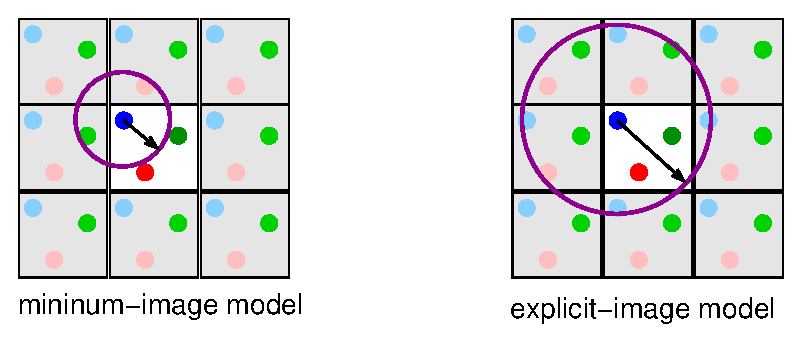
\includegraphics{min_im.eps}\end{center}


\caption{\label{cap:1}3- and 2-D periodic models}
\end{figure}


Molecular mechanics module uses \texttt{\textbf{periodic boundary
conditions}} in a combination with two different image conventions
to calculate interactions between atoms (species) forming simulated
molecular system: the \texttt{\textbf{minimum image}}\cite{allen}
method and the \texttt{\textbf{explicit image}} one (figure \ref{cap:1}).
The first method means that only one - the nearest \={ } image of
each species is used to calculate short-range bonded and non-bonded
interactions and also real-space part of Coulomb sum implemented in
the frameworks of Ewald method. Using the \texttt{\textbf{minimum
image}} method for estimation of bonded covalent interaction terms
is always justified due to their very local character. On the contrary,
non-bonded interactions like van der Waals potentials or electrostatic
real-space part of Ewald method are not local. Their calculation are
based on cut-off radius $R_{cut}$. For such interaction terms the
\texttt{\textbf{minimum image}} method implies that the cut-off radius
$R_{cut}$ used to truncate non-bonded interactions must not exceed
half the shortest unit cell vector\begin{equation}
R_{cut}<\frac{1}{2}\min\left(a,b,c\right)\label{eq:33}\end{equation}
otherwise more then one atom image would be found within cut-off distance.

The \texttt{\textbf{minimum image}} method is a very suitable to be
applied to systems, like molecular crystals or proteins in solution,
having large unit (simulation) cell or boxes. The main advantage of
the method is saving memory because the maximal (generally unreachable)
dimension size of non-bonded \texttt{\textbf{pair list}} for each
atom cannot exceed the total number of species of simulated system.
But, in general, ionic or covalent solid crystals have length of unit
cell vectors smaller than usual value of cut-off radius ($\sim8\div12$
�). In this case Molecular mechanics module applies the \texttt{\textbf{explicit
image}} method, which implies that to calculate non-bonded interactions
all images of each species $j$ that satisfies the condition $\left|\overrightarrow{r}_{j}-\overrightarrow{r}_{i}\right|\leq R_{cut}$
have to be considered (figure \ref{cap:1}). To use the last approach
a construction of non-bonded \texttt{\textbf{pair lists}} has to be
modified. Now non-bonded \texttt{\textbf{pair lists}} contain not
only numbers of real atoms of system but numbers of images satisfied
the cut-off condition.


\subsection{Strain tensor and strain derivatives}

~~~~~Periodic system like crystal lattice in non-equilibrium
states always is influenced by internal stretching or compressing
forces which can alter parameters of unit cell\cite{catlow82,taylor}.
For small deformation $\overrightarrow{\partial u}=\left(\partial u_{x},\partial u_{y},\partial u_{z}\right)$
any vector $\overrightarrow{r}$ in a crystal lattice becomes a vector
$\overrightarrow{r}^{\prime}$ as follows:\begin{eqnarray}
r_{x}^{\prime} & = & \left(1+\frac{\partial u_{x}}{\partial r_{x}}\right)r_{x}+\frac{\partial u_{y}}{\partial r_{y}}r_{y}+\frac{\partial u_{z}}{\partial r_{z}}r_{z}\nonumber \\
r_{y}^{\prime} & = & \frac{\partial u_{x}}{\partial r_{x}}r_{x}+\left(1+\frac{\partial u_{y}}{\partial r_{y}}\right)r_{y}+\frac{\partial u_{z}}{\partial r_{z}}r_{z}\label{eq:21}\\
r_{z}^{\prime} & = & \frac{\partial u_{x}}{\partial r_{x}}r_{x}+\frac{\partial u_{y}}{\partial r_{y}}r_{y}+\left(1+\frac{\partial u_{z}}{\partial r_{z}}\right)r_{z}\nonumber \end{eqnarray}
 or in matrix form:\begin{equation}
\overrightarrow{r}^{\prime}=\left(\overline{\overline{I}}+\overline{\overline{\epsilon}}\right)\cdot\overrightarrow{r}\label{eq:22}\end{equation}
$\overline{\overline{\epsilon}}$ in equation \ref{eq:22} is the
strain tensor with elements \begin{eqnarray}
\nonumber \\\epsilon_{ij} & = & \frac{1}{2}\left(\frac{\partial u_{i}}{\partial r_{j}}+\frac{\partial u_{j}}{\partial r_{i}}\right)\label{eq:23}\end{eqnarray}
The $3\times3$ strain tensor $\overline{\overline{\epsilon}}$ is
symmetric and has only 6 independent elements defined as\begin{equation}
\overline{\overline{\epsilon}}=\left(\begin{array}{ccc}
\epsilon_{1} & \frac{\epsilon_{6}}{2} & \frac{\epsilon_{5}}{2}\\
\frac{\epsilon_{6}}{2} & \epsilon_{2} & \frac{\epsilon_{4}}{2}\\
\frac{\epsilon_{5}}{2} & \frac{\epsilon_{4}}{2} & \epsilon_{3}\end{array}\right)\label{eq:24}\end{equation}
From equation \ref{eq:22}\begin{equation}
r^{\prime2}=r^{2}+2\cdot\overrightarrow{r}^{\top}\cdot\overline{\overline{\epsilon}}\cdot\overrightarrow{r}+\overrightarrow{r}^{\top}\cdot\overline{\overline{\epsilon}}^{2}\overrightarrow{r}\label{eq:24}\end{equation}
here $r=\left|\overrightarrow{r}\right|$. Equation \ref{eq:24} is
used to obtain energy derivatives in respect to elements of strain
tensor. Near the equilibrium positions (at zero strain) the following
first derivatives can be derived:\begin{equation}
\frac{1}{2}\frac{\partial r^{2}}{\partial\epsilon_{i}}=r_{k}r_{l}\; for\;\left\{ \begin{array}{c}
i=1,2,3,4,5,6\\
k=x,y,z,y,x,x\\
l=x,y,z,z,z,y\end{array}\right.\label{eq:25}\end{equation}
Thus, for a pair potential $U=\Phi(r)$ in which $r=\left|\overrightarrow{r_{1}}-\overrightarrow{r_{2}}\right|$:
\begin{eqnarray}
\frac{\partial U}{\partial\epsilon_{i}} & = & \frac{\partial\Phi\left(r\right)}{\partial r}\frac{\partial r}{\partial\epsilon_{i}}\nonumber \\
 & = & \frac{\partial\Phi\left(r\right)}{\partial r}\frac{1}{2r}\frac{\partial r^{2}}{\partial\epsilon_{i}}\label{eq:26}\\
 & = & V\left(r\right)r_{k}r_{l}\nonumber \end{eqnarray}
Here $V\left(r\right)=\frac{\partial\Phi\left(r\right)}{r\partial r}$.
In the same way anyone can derive strain derivatives for 3-body interactions
$U=U\left(\theta\right)=\Phi\left(\overrightarrow{r_{1}},\overrightarrow{r_{2}},\overrightarrow{r_{3}}\right)$:\begin{equation}
\frac{\partial U}{\partial\epsilon_{i}}=V1\left(\overrightarrow{r_{1}},\overrightarrow{r_{2}},\overrightarrow{r_{3}}\right)r_{1k}r_{1l}+V2\left(\overrightarrow{r_{1}},\overrightarrow{r_{2}},\overrightarrow{r_{3}}\right)r_{2k}r_{2l}+V3\left(\overrightarrow{r_{1}},\overrightarrow{r_{2}}\right)r_{3k}r_{3l}\label{eq:27}\end{equation}
in which \begin{equation}
\begin{array}{ccc}
V1\left(\overrightarrow{r_{1}},\overrightarrow{r_{2}},\overrightarrow{r_{3}}\right) & = & -\frac{1}{\sin\theta}\frac{\partial U}{\partial\theta}\frac{\overrightarrow{r_{1}}^{2}-\overrightarrow{r_{2}}^{2}+\overrightarrow{r_{3}}^{2}}{2\cdot r_{1}^{3}\cdot r_{2}}\\
V2\left(\overrightarrow{r_{1}},\overrightarrow{r_{2}},\overrightarrow{r_{3}}\right) & = & -\frac{1}{\sin\theta}\frac{\partial U}{\partial\theta}\frac{\overrightarrow{r_{2}}^{2}-\overrightarrow{r_{1}}^{2}+\overrightarrow{r_{3}}^{2}}{2\cdot r_{2}^{3}\cdot r_{1}}\\
V3\left(\overrightarrow{r_{1}},\overrightarrow{r_{2}}\right) & = & \frac{1}{\sin\theta}\frac{\partial U}{\partial\theta}\frac{1}{r_{1}\cdot r_{2}}\end{array}\label{eq:28}\end{equation}
To calculate strain derivatives of the reciprocal part of the Ewald
summation anyone has to differentiate reciprocal lattice vectors in
respect to elements of a strain tensor:\begin{equation}
-\frac{1}{2}\frac{\partial k^{2}}{\partial\epsilon_{i}}=k_{k}k_{l}\; for\;\left\{ \begin{array}{c}
i=1,2,3,4,5,6\\
k=x,y,z,y,x,x\\
l=x,y,z,z,z,y\end{array}\right.\label{eq:29}\end{equation}
and corresponding first strain derivatives of the Coulomb energy in
the reciprocal space $U_{recip}\left(\overrightarrow{k},\overrightarrow{r}\right)$
are equal\begin{eqnarray}
\frac{\partial U_{recip}\left(\overrightarrow{k},\overrightarrow{r}\right)}{\partial\epsilon_{i}} & = & -\frac{1}{\varepsilon_{0}V}\sum_{\overrightarrow{k}>0}\frac{\exp\left(-\frac{k^{2}}{4\alpha^{2}}\right)}{k^{2}}\left\{ \left|\sum_{i=1}^{N}q_{i}\cos\left(\overrightarrow{k}\cdot\overrightarrow{r_{i}}\right)\right|^{2}\right.\nonumber \\
 & + & \left.\left|\sum_{i=1}^{N}q_{i}\sin\left(\overrightarrow{k}\cdot\overrightarrow{r_{i}}\right)\right|^{2}\right\} \left[\delta_{kl}-2\left(\frac{1}{k^{2}}+\frac{1}{4\alpha^{2}}\right)k_{k}k_{l}\right]\label{eq:30}\end{eqnarray}


Second derivatives of system energy in respect to strain are naturally
more complicated and can be found elsewhere (\cite{catlow82,taylor}).
Also this manual pays no special attention to strain derivatives of
2-D periodic systems, because two-dimensional strain is only a special
case of strain tensor of systems with periodicity in three directions. 


\section{Geometry optimization}

~~~~~In the current version of Molecular mechanics module a calculation
of system configuration with minimal energy is the main part of the
program. There are variety of geometry optimization methods distinguished
by an information used and speed of convergence to reach minimum,
usually a local minimum. Unfortunately, no method exists that can
guarantee the determination of the global minimum in any reasonable
amount of time, even for relatively small system containing about
hundred species. All existed methods of searching minimum can be divided
into three groups:

\begin{enumerate}
\item Methods that require only function calculations. The most popular
are the \texttt{\textbf{simplex}} method and its variants. To calculate
a next step results of previous evaluation are used.
\item Methods that use an information on first derivatives (gradient). This
is the most varied part of optimization methods. The \texttt{\textbf{steepest
descent}} method simply performs a step in the direction of the negative
gradient. The \texttt{\textbf{conjugate gradient}} method has a faster
convergence because to calculate a next step it uses gradient information
obtained from previous steps. The most fast converging methods based
on gradient information are \texttt{\textbf{quasi-Newton}} ones. The
basic idea of these methods is building up curvature information progressively.
Before calculation of a next step, the current approximation to the
direct or inverse Hessian is updated by using new gradient information.
\item The \texttt{\textbf{Newton-Raphson}} methods that use second information
as well. These methods have the fastest convergence but the problem
is that for $N$ species consisting modeled system the Hessian matrix
$3N\times3N$ must be computed, stored and inverted.
\end{enumerate}
~~~~~Because of a calculation of energy second derivatives are
among the main program abilities and available for all types of interactions,
and current size of modeled system hardly can exceed one-two thousand
atoms, Molecular mechanics module exploits a combination of \texttt{\textbf{quasi-Newton}}
and \texttt{\textbf{Newton-Raphson}} methods. It means that any user
has a possibility to choose between a constructing Hessian from analytical
second derivatives or using a diagonal matrix as initial Hessian form,
between calculating Hessian at each geometry step (\texttt{\textbf{Newton-Raphson}}
method) or its updating during some steps using \texttt{\textbf{BFGS\cite{schlegel}}}
scheme. 

\texttt{\textbf{BFGS}} scheme \begin{eqnarray}
\overline{\overline{H}}_{k}^{-1} & = & \left[\overline{\overline{I}}-\frac{\Delta\overrightarrow{x}_{k}\Delta\overrightarrow{g}_{k}^{\top}}{\Delta\overrightarrow{x}_{k}^{\top}\cdot\Delta\overrightarrow{g}_{k}}\right]\overline{\overline{H}}_{k-1}^{-1}\left[\overline{\overline{I}}-\frac{\Delta\overrightarrow{x}_{k}\Delta\overrightarrow{g}_{k}^{\top}}{\Delta\overrightarrow{x}_{k}^{\top}\cdot\Delta\overrightarrow{g}_{k}}\right]^{\top}\label{eq:34}\\
 & + & \frac{\Delta\overrightarrow{x}_{k}\Delta\overrightarrow{x}_{k}^{\top}}{\Delta\overrightarrow{x}_{k}^{\top}\cdot\Delta\overrightarrow{g}_{k}}\nonumber \end{eqnarray}
was chosen because approximate Hessian produced is always positive-defined
and, consequently, each geometry step $k$ leads to energy minimum.\begin{equation}
\Delta\overrightarrow{x}_{k}=-\overline{\overline{H}}_{k}^{-1}\cdot\overrightarrow{g}_{k}\label{eq:35}\end{equation}


Geometry optimization of non-periodic system is carried out in Cartesian
coordinates. Optimization of periodic systems also can be done in
Cartesian coordinates but simultaneous optimization of unit cell parameters
in this case produce some problems that are due to dependence atom
Cartesian coordinates on elements of the strain tensor(eq. \ref{eq:22}).
On the contrary, fractional (internal) coordinates are absolutely
independent on the strain tensor and, as consequence, parameters of
unit cell. That is why, geometry optimization of periodic system goes
in fractional (internal) coordinates(figure \ref{cap:3}).%
\begin{figure}
\begin{center}\includegraphics[%
  width=0.40\textwidth,
  height=0.60\textwidth]{opt.eps}\end{center}


\caption{\label{cap:3} Single step of optimization of periodic systems}
\end{figure}



\subsection{Hessian evaluation}

~~~~~Optimization process based on using the inverse Hessian
of system. Firstly the matrix of second derivatives is calculated.
It has size $\left(3N+nst\right)\times\left(3N+nst\right)$. Here
$nst$ is the number of strain variable used. It is equal zero if
no periodicity or no optimization of unit cell parameters, otherwise
$nst$ is equal 3 or 6 for 2- or 3-D periodic systems, correspondingly.
The memory to hold such a great matrix is used dynamically and fried
during optimization steps and inverse Hessian updating. The inverse
Hessian is used whole optimization process and to save memory it is
stored in packed form (upper triangle)

The main problem of systems optimized in Cartesian coordinates is
a inversion of direct Hessian. It is a sixfold singular due to external
degrees of freedom (translations and rotations). That is why to optimize
non-periodic systems instead of standard BLAS or LAPACK routines the
so-called \texttt{\textbf{generalized inverse}} procedure\cite{worshel,white}
was implemented. \texttt{\textbf{Generalized inversion}} means that
inverse matrix $\overline{\overline{H}}^{-1}$ is constructed from
eigenvalues $\left(\lambda\right)$ and eigenvectors $\overrightarrow{E}$
of the direct matrix $\overline{\overline{H}}$. Following this approach
matrix $\overline{\overline{H}}^{-1}=\overrightarrow{E}\cdot\overline{\overline{\Lambda}}^{-1}\cdot\overrightarrow{E}^{\top}$.
The matrix $\overline{\overline{\Lambda}}^{-1}$ is diagonal whose
elements are formed from eigenvalues : $\overline{\overline{\Lambda}}_{ii}^{-1}=1/\lambda_{i}\:\left(\lambda_{i}\neq0\right)$
and $\overline{\overline{\Lambda}}_{jj}^{-1}=0\:\left(\lambda_{j}=0\right)$.

Periodic systems have no rotational degrees of freedom but translations
are still exist. To eliminate translating degrees of freedom one constrain
is imposed on optimized periodic system. The first atom (species)
is considered to be fixed. Now whole system consists of $3N+nst-3$
degrees of freedom and a final direct Hessian can be inverted without
any problem by standard LAPACK routines.


\subsection{Line search}

~~~~~\texttt{\textbf{Line search}} is strong necessary if optimization
is performed in Cartesian or fractional (internal) coordinates to
find real energy minimum along calculated geometry step, otherwise
reduction of calculated geometry step by factor of $\sim0.1$ is often
required. That is why, \texttt{\textbf{line search}} can great reduce
number of evaluating function. Two algorithms of \texttt{\textbf{line
search}} were implemented. The first method is based on fitting a
cubic parabola to the energy and gradient at $\overrightarrow{x}_{k}$
and $\overrightarrow{x}_{k}+\Delta\overrightarrow{x}_{k}$, and calculating
the energy at cubic parabola minimum (figure \ref{cap:4}a).%
\begin{figure}
\begin{center}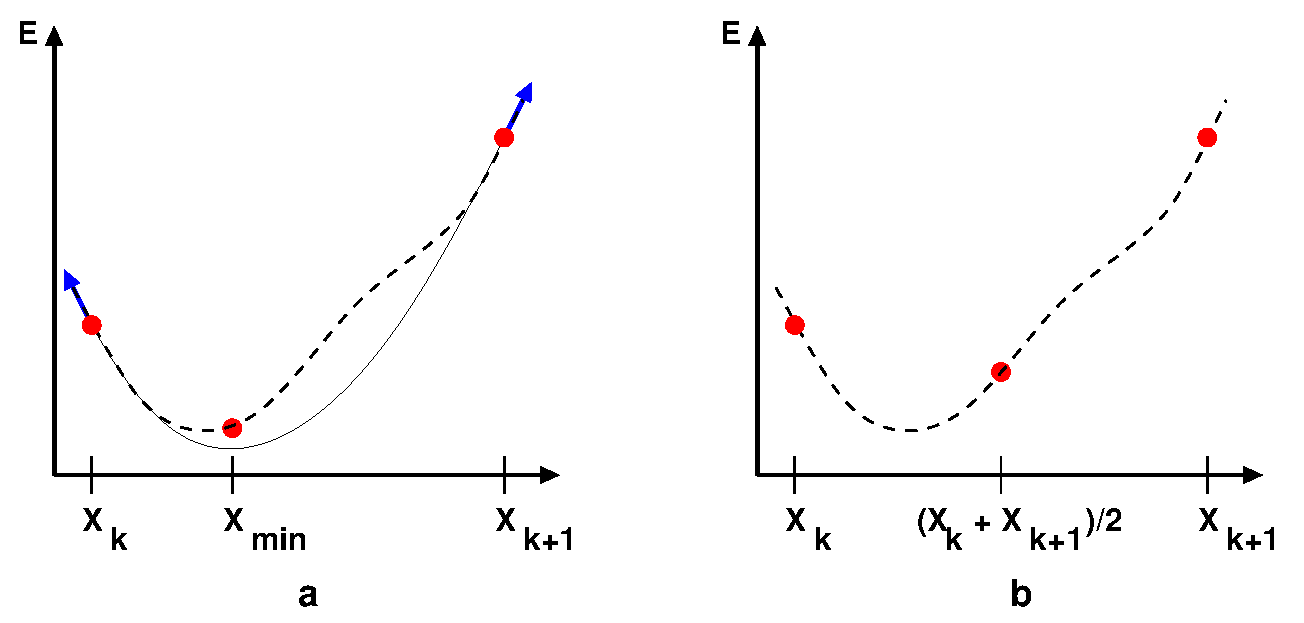
\includegraphics[%
  width=0.80\textwidth,
  height=0.25\textwidth]{linesearch.eps}\end{center}


\caption{\label{cap:4} Line search methods: a) fitting cubic parabola; b)
half dividing geometry step}
\end{figure}
 The second one does not calculate gradient at all and uses only energy
values. It can be called as \texttt{\textbf{half dividing step}} (figure
\ref{cap:4}b). Algorithms of both \texttt{\textbf{line searches}}
presented on the figure \ref{cap:5}.%
\begin{figure}
\begin{center}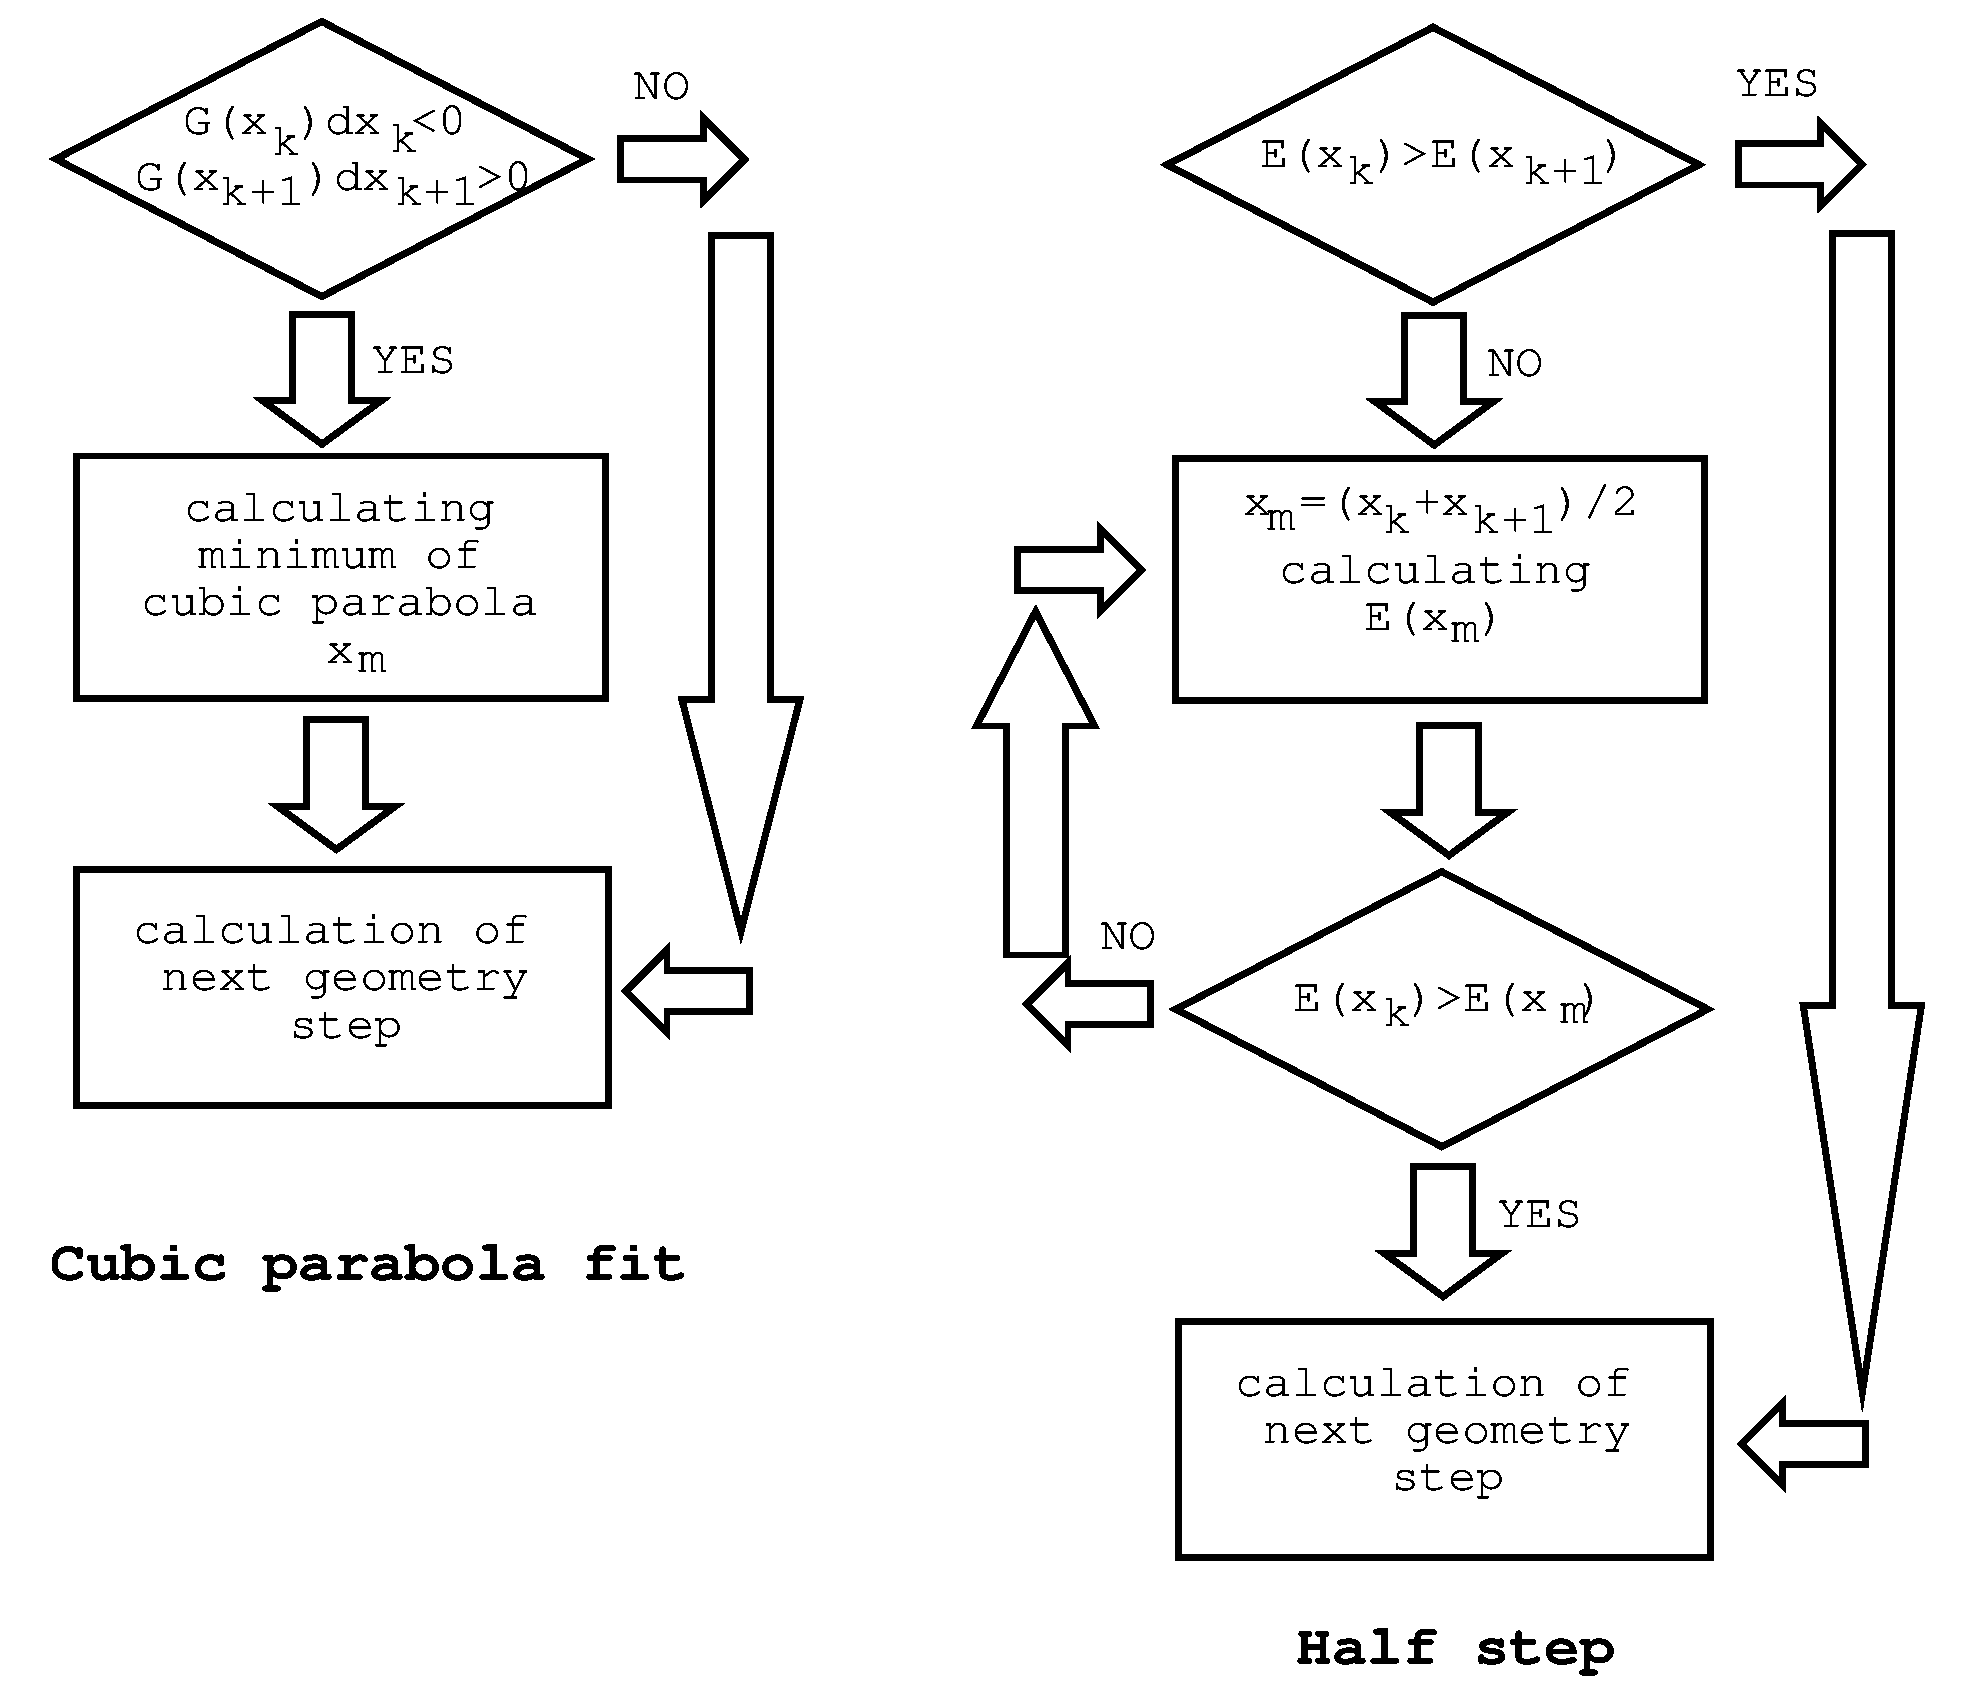
\includegraphics[%
  width=0.70\textwidth,
  height=0.40\textwidth]{lsfd.eps}\end{center}


\caption{\label{cap:5}Line search algorithms}
\end{figure}
 Both methods have advantages and disadvantages. Fitting cubic parabola
usually allows to reduce total number of geometry steps to reach energy
minimum of system, in the contrary, the second variant can be less
time expensive for large system due to no gradient evaluating. 


\section{Parallelization of reciprocal-space Ewald sum}

~~~~~Calculating electrostatic interaction of periodic systems
by Ewald method is one of the most time consumable tasks but real\={ }
and reciprocal-space parts of Ewald equations (\ref{eq:19},\ref{eq:20})
have different scaling. For a fixed parameter $\alpha$ and accuracy
the number of terms in the real-space sum is proportional to the total
number $N$ of system species but the reciprocal-space sum scales
as $N^{3/2}$ for 3-D Ewald method or $N^{2}$ for 2-D variant. The
difference of scaling between two variants of Ewald method springs
from the fact that the pair separation, $\overrightarrow{r}_{ij}$,
in reciprocal part of equation \ref{eq:20} are no longer separable
because of the necessity to decouple the aperiodic $z$ component
from the periodic $x$ and $y$ components\cite{joannis}. Therefore,
the complexity of 2-D Ewald method results worse scaling. Fortunately,
worse scaling of 2-D Ewald method in comparison with 3-D one can be
sometime compensated by smaller number of reciprocal lattice vectors. 

To compensate not optimal scaling of the reciprocal-space part of
Ewald method, it was implemented in a parallel manner. Distinctions
between 3-D and 2-D reciprocal-space summations imply using different
methods of parallelization. Following equation \ref{eq:19} 3-D reciprocal-space
summation is parallelized in accordance with reciprocal lattice vectors
$k$. That is, each processor $i$ calculate parts of total energy,
gradients and second derivatives (if required) corresponding its own
part of reciprocal lattice vectors $k_{i}$. 

Parallelization of 2-D reciprocal-space summation was done in correspondence
with atom index. It implies each processor $i$ calculates a contribution
to reciprocal-space summation due to owned atoms. The double summation
in equation \ref{eq:20} due to necessity to calculate all possible
inter-atomic distances, $\overrightarrow{r}_{ij}$, between all atoms
of unit cell. It can be presented as quadratic matrix (figure \ref{cap:6}
a, b).%
\begin{figure}
\begin{center}\includegraphics{fm.eps}\end{center}


\caption{\label{cap:6}Algorithms of calculation inter-atomic distances in
the reciprocal-space part of 2-D Ewald summation.}
\end{figure}
 To avoid double accounting and save computer time only half of such
matrix should be calculated. In this case the most important thing
is to provide effective load-balancing. The variant $a$ run effectively
on a single processor node. That is why it has to be modified to be
able to be execute as a parallel job on many processor machines. When
the upper right triangle of the matrix is reflected to the lower left
triangle (variant $b$), all possible distances, $\overrightarrow{r}_{ij}$
, can be still calculated but now every processor $i$ in the matrix
computes almost the same number of possible distances and corresponding
contributions to the total energy, gradients and second derivatives.

To perform a next Newton step of geometry optimization all required
data (gradients and second derivatives) has to be collected and summed
up on the master processor. For large modeled systems, especial if
second derivatives to be required, a point-to-point communications
of each processor with muster one can lead to parallel overhead. That
is, the program executing can be stopped until the master processor
has received the data flow from its slaves. To avoid the described
situation a cascade procedure developed in \noun{ParaGauss} package
\cite{norte} was implemented to gather gradient and Hessian data.

\begin{thebibliography}{10}
\bibitem{mm3}N. L. Allinger, Y. H. Yuh, J.-H. Lii, J. Am. Chem.Soc., 111, 8551-8566
(1989) 
\bibitem{ewald3}P. P. Ewald, Ann. Physik, 64, 253 (1921)
\bibitem{parry}D. E. Parry, Surface Sci., 49, 433 (1975)
\bibitem{ewald2}D. M. Hayes, M. Barber, J. H. R. Clarke, J. Chem. Soc. Faraday Trans.
II, 73, 1485-1496 (1977)
\bibitem{fincham}D. Fincham, Mol. Simulation, 8, 165-178 (1992)
\bibitem{jackson}R. A. Jackson, C. R. A. Catlow, Mol. Simulation, 1, 207 (1988)
\bibitem{mm2}N. L. Allinger, J. Am. Chem.Soc., 99, 8127 (1977)
\bibitem{catlow82}C. R. A. Catlow, W. C. Mackrodt, in Computer Simulation of Solids,
edited by C. R. A. Catlow, W\.{ } C. Mackrodt, Lecture Notes in Physics
166, Springer-Verlag\c{ } Berlin, 1982, 3-20
\bibitem{taylor}M. B. Taylor, G. D. Barrera, N. L. Allan, T. H. K. Barron, Phys. Rev.
B, 56, 14380-14390 (1997)
\bibitem{dl_poly}W. Smith, T. R. Forester, DL\_POLY\_2 User Manual, version 2.12, CCRLC,
Daresbury Laboratory, Daresbury, Warrington, WA4 4AD, England, 1999 
\bibitem{charmm}B. R. Brooks, R. E. Bruccoleri, B. D. Olafson, D. J. States, S. Swaminathan,
M. Karplus, CHARMM: A Program for Macromolecular Energy, Minimization,
and Dynamics Calculations, J. Comp. Chem. 4, 187-217 (1983)
\bibitem{gromacs}D. van der Spoel, A. R. van Buuren, E. Apol, P. J. Muelenhoff, D.
P. Tielemann, A. L. T. M. Sijbers, B. Hess, K. A. Feenstra, E. Lindahl,
R. van Drunen, H. J. C. Berendsen, GROMACS User Manual, version 3.1.1,
Department of Biophysical Chemistry, University of Groningen, Nijenborgh
4, 9747 AG Groningen, The Netherlands, 1999-2001 
\bibitem{amber}D. A. Case, D. A. Pearlman, J. W. Caldwell, T. E. Cheatham III, J.
Wang, W. S. Ross, C. Simmerling, T. Darden, K. M. Merz, R. V. Stanton,
A. Cheng, J. J. Vincent, M. Crowley, V. Tsui, H. Gohlke, R. Radmer,
Y. Duan, J. Pitera, I. Massova, G. L. Seibel, U. C. Singh, P. Weiner,
P. A. Kollman, AMBER 7, University of California, San Francisco, 2002
\bibitem{ego}M. Eichinger, H. Grubm\"{u}ller, H. Heller, User Manual for EGO\_VIII
(release 2.0), Leibniz-Rechenzentrum der Bayerischen Akademie der
Wissenschaften, M\"{u}nchen, Germany, 1995
\bibitem{worshel}A. Worshel, S. Lifson, J. Phys. Chem., 53, 582-594 (1970) 
\bibitem{white}D. N. J. White, Acta Cryst., A33, 1010-1011 (1977) 
\bibitem{allen}M. P. Allen, D. J. Tildesley, Computer simulation of liquids, Clarendon
Press, Oxford Science Publications (1987)
\bibitem{schlegel}H. B. Schlegel, in Ab Initio Methods in Quantum Chemistry, V1, edited
by K. P. Lawley, John Wiley \& Sons Ltd., 1987
\bibitem{joannis}J. de Joannis, A. Arnold, C. Holm, J. Phys. Chem., 117, 2503-2512
(2002)
\bibitem{norte}F. C. N�rtemann, A Parallel implementation of the density functional
method. SCF part, optimization package and application to gold cluster,
PhD Thesis, Technische Universit�t, M\"{u}nchen, Germany, 1998
\end{thebibliography}

\end{document}
